 
   %judul bisa diketik ulang
  \setstretch{1}%\small
  \begin{center}
      \textbf{\large \Title}\\
      \bigskip 
  \end{center}
  
  
  
  %Nama authors
   \begin{center}
     \bf \Author$^1$, Ade Romadhony$^2$
  \end{center}
  
  
  %Afiliasi dan email
   \begin{center}
      $^{1,2}$Fakultas Informatika, Universitas Telkom, Bandung\\
      $^1$nurcahyo@student.telkomuniversity.ac.id, $^2$aderomadhony@telkomuniversity.ac.id
  \end{center}
  
   
 %%% Abstrak Indonesia %%%%%%%%%%  
   
{\bf \parindent0pt \noindent\rule{\textwidth}{1pt}
Alat anotasi yang tersedia untuk \textit{combinatory categorial grammar} (CCG) masih sangat terbatas.
Salah satu aplikasi dengan antarmuka grafis yang dapat digunakan adalah CCGweb. Untuk dapat
menggunakan CCGweb, pengguna diharuskan untuk melakukan \textit{setup} secara mandiri. Proses ini
dapat menjadi keterbatasan bagi \textit{annotator} karena \textit{dependency} yang perlu
dipersiapkan cukup banyak. Selain itu, CCGweb hanya dapat mengerjakan satu proyek anotasi CCG
dalam satu waktu. Demikian itu, kami membangun alat anotasi CCG yang dapat langsung digunakan
oleh pengguna tanpa perlu melakukan \textit{setup} terlebih dahulu. Alat anotasi tersebut kami
beri nama CCGtown. Dengan CCGtown, pengguna dapat membuat banyak proyek anotasi sekaligus dan
telah dilengkapi fitur yang sebagian besarnya tersedia di CCGweb. CCGtown merupakan alat anotasi
CCG alternatif yang dapat digunakan oleh \textit{annotator} CCG.


\bigskip
Kata kunci: pemrosesan bahasa alami, combinatory categorial grammar, alat anotasi



%%% Abstrak English %%%%%%%%%%  



\noindent\rule{\textwidth}{1pt}
Abstract

Annotation tools available for combinatory categorial grammar (CCG) are still limited.
One of the annotation tool with a graphical interface that can be used is CCGweb.
To be able to use CCGweb, users are required to setup independently.
This process can be a limitation for annotators because of the many dependencies that
need to be prepared.
CCGweb also can only work on one CCG annotation project at a time.
With that in mind, we built a CCG annotation tool that users can use right away without
any setup required.
We call the annotation tool CCGtown.
With CCGtown, users can create multiple annotation projects at once and it has features
that are mostly available on CCGweb.
CCGtown is an alternative CCG annotation tool which can be used by CCG annotators.


\bigskip
Keywords: natural language processing, combinatory categorial grammar, annotation tool

\noindent\rule{\textwidth}{1pt} }
   


%%%%%% isi paper %%%%

\section{Pendahuluan}

\noindent\textbf{Latar Belakang}

CCGweb\footnote{\url{https://github.com/texttheater/ccgweb}} merupakan alat anotasi
\textit{open source} berbasis web pertama yang dikembangkan khusus untuk memberikan anotasi
CCG\citep{evang-etal-2019-ccgweb}. Fitur yang ditawarkan CCGweb cukup beragam mulai dari
\textit{dynamic annotation}, WYSIWYG (\textit{what you see is what you get}),
\textit{lexical category constraint}, \textit{span constraint}, \textit{issue reporting} via
layanan \textit{web service} eksternal, hingga \textit{adjudication support}. Selain itu, CCGweb
dibangun untuk membangun \textit{dataset} CCG \textit{multilingual} yang artinya terdapat lebih
dari satu bahasa untuk satu kalimat yang sama. Untuk dapat menggunakan CCGweb, pengguna harus
melakukan instalasi manual secara mandiri dan dapat dilakukan baik di komputer pribadinya ataupun
di layanan \textit{hosting} maupun \textit{cloud}. Adapun proyek anotasi yang dapat dikerjakan
dalam satu waktu adalah satu buah proyek yang mana dapat memiliki satu bahasa atau lebih.
Demikian itu, pengguna tidak dapat mengerjakan lebih dari satu proyek dan harus menyelesaikan
proyek sebelumnya agar dapat memulai proyek baru. Alternatif lainnya adalah melakukan instalasi
kembali sehingga pengguna akan memiliki lebih dari satu aplikasi CCGweb.

Untuk dapat menggunakan CCGweb, pengguna diharapkan telah mempersiapkan beberapa
\textit{dependency} yang diperlukan yaitu
EasyCCG\footnote{\url{https://github.com/ParallelMeaningBank/easyccg}} (termasuk berkas modelnya),
Elephant \textit{tokenizer}\footnote{\url{https://github.com/ParallelMeaningBank/elephant}}
(termasuk berkas modelnya), berkas model UDPipe\footnote{\url{https://ufal.mff.cuni.cz/udpipe}},
Produce \textit{build system}\footnote{\url{https://github.com/texttheater/produce}}, dan
Viasock\footnote{\url{https://github.com/texttheater/viasock}}. Selain \textit{dependency} tersebut,
beberapa \textit{dependency} lainnya relatif mudah untuk dipersiapkan sehingga dapat kita lewati.
Kelima \textit{dependency} yang diperlukan tersebut harus dipersiapkan secara mandiri. Hal ini
menyulitkan bagi pengguna yang ingin menggunakan CCGweb di komputer pribadinya karena proses ini
rawan mengalami \textit{error} seperti perbedaan versi yang digunakan antar \textit{dependency}-nya
dan sebagainya. Kendala yang dialami oleh calon pengguna ketika melakukan \textit{setup} juga dapat
mengurangi minat calon kontributor untuk memberikan kontribusi bagi pengembangan CCGweb. Demikian
itu, langkah \textit{setup} yang perlu dilakukan sebaiknya dikurangi hingga sesedikit mungkin.
Salah satu solusinya adalah dengan menambahkan perintah baru untuk melakukan otomasi proses
\textit{setup} seperti menyiapkan semua \textit{dependency} yang diperlukan secara otomatis,
melakukan instalasi DBMS\footnote{\textit{database management system}} secara otomatis, membuatkan
tabel-tabel yang diperlukan secara otomatis, dan seterusnya. Akibatnya, calon pengguna dan calon
kontributor dapat langsung fokus pada tujuannya dalam menggunakan alat anotasi tersebut tanpa perlu
direpotkan untuk melakukan \textit{setup} yang panjang.

CCGtown\footnote{\url{https://github.com/wisn/ccgtown}} merupakan alat anotasi CCG alternatif yang
dapat digunakan oleh \textit{annotator}. CCGtown memiliki kemampuan untuk membuat banyak proyek
anotasi sekaligus. Selain itu, CCGtown juga dapat langsung digunakan secara daring tanpa perlu
melakukan instalasi terlebih dahulu. Untuk memudahkan calon kontributor, CCGtown menggunakan
\textit{web framework} populer yang dapat dipelajari oleh siapapun serta menyediakan
perintah-perintah yang dapat digunakan untuk melakukan otomasi seperti contohnya pada proses
\textit{setup}-nya. CCGtown juga dipublikasikan sebagai \textit{open source software} sehingga
siapapun dapat melihat sumber kodenya, menambahkan fitur, mengurangi fitur, mengunggah CCGtown di
\textit{server} pribadinya, dan masih banyak lagi. Adapun fitur yang dimiliki CCGtown saat ini
mirip dengan CCGweb hanya saja dengan beberapa penyesuaian. Pengguna dapat menambahkan banyak
proyek sekaligus, dapat menambahkan kalimat yang ingin diberikan anotasi, dapat memberikan anotasi
CCG, dapat menyunting CCG \textit{derivation} secara langsung dengan konsep WYSIWYG, dapat
melakukan \textit{generate} CCG \textit{derivation}, dan dapat melakukan \textit{auto-assign} CCG
\textit{lexicon}. Fitur-fitur lainnya dapat ditambahkan di lain waktu.
\\


\noindent\textbf{Topik dan Batasannya}

Anotasi berdasarkan KBBI merupakan sebuah \textit{catatan} yang dibuat oleh pengarang atau
orang lain untuk menerangkan, mengomentari, atau mengkritik teks karya sastra atau
bahan tertulis lain. Dalam konteks pemrosesan bahasa alami, anotasi merupakan sebuah
\textit{catatan} yang digunakan untuk merepresentasikan suatu makna tertentu.
Representasi tersebut umumnya sesuatu yang dapat "dipahami" oleh komputer.
Sebagai contoh, pada kalimat "Pamungkas kemarin makan rendang" kita dapat memberikan anotasi
"Pamungkas[ORANG] kemarin makan rendang[MAKANAN]". Maksud dari anotasi tersebut yaitu "Pamungkas"
dalam kalimat tersebut merupakan representasi dari orang sebagai subjeknya dan "rendang"
merupakan representasi dari makanan sebagai objeknya. Memberikan anotasi secara manual merupakan
kegiatan yang melelahkan. Demikian itu, alat anotasi dikembangkan untuk membantu meringankan
proses pemberian anotasi.

Alat anotasi untuk pemrosesan bahasa alami yang tersedia sejatinya sudah cukup banyak.
Jenis, kemampuan, dan biaya masing-masing alat anotasi tersebut juga beragam. Sebagai contoh,
tagtog\footnote{\url{https://tagtog.net/}} merupakan alat anotasi berbasis web yang dapat digunakan
secara gratis maupun berbayar. Selain tagtog, prodigy\footnote{\url{https://prodi.gy/}} juga
merupakan alat anotasi berbasis web tetapi tidak dapat digunakan secara gratis. Selain itu, prodigy
mendukung lebih banyak tipe anotasi seperti Named Entity, POS Tagging, Dependency Parsing,
dan lain-lain. Kendati banyaknya alat anotasi yang sudah tersedia, dukungan anotasi untuk
Combinatory Categorial Grammar (CCG) belum banyak. Salah satu alat anotasi CCG dengan antarmuka
grafis yang tersedia adalah CCGweb\footnote{\url{https://ccgweb.phil.hhu.de/}}.

Anotasi CCG sebenarnya memiliki bentuk yang rumit. Anotasi CCG memiliki bentuk sintaktik dan
bentuk semantik. Bentuk $(S/N)$ yang akan dilihat pada bagian selanjutnya merupakan bentuk sintaktik
dari CCG\citep{Lambek1988}. Adapun $: \lambda x.\lambda y.\ suka(y, x)$ yang akan dilihat pada bagian
selanjutnya merupakan bentuk semantik dari CCG. Bentuk sintaktik CCG sejatinya juga dapat lebih
kompleks ketimbang hanya memiliki bentuk $(S/N)$ saja. Akan tetapi, CCGtown saat ini ekspektasinya
hanya dapat digunakan untuk anotasi CCG yang bentuknya sederhana. Hal tersebut dikarenakan terbatasnya
sumber \textit{dataset} yang dapat dijadikan sampel. Salah satu \textit{dataset} yang dapat digunakan
adalah CCGbank. Namun, CCGbank bukanlah \textit{dataset} yang dapat dengan bebas diperoleh.
Demikian itu, CCGtown menggunakan sampel yang tersedia secara terbuka saja seperti contoh kasus
dari referensi yang digunakan, contoh anotasi CCG di halaman NLTK, dan sebagainya.

Fokus CCGtown pada Tugas Akhir ini adalah untuk memberikan alternatif alat anotasi CCG yang telah
tersedia yaitu CCGweb. CCGtown menyuguhkan \textit{development cycle} yang lebih baik dari CCGweb
dan menyediakan perintah-perintah untuk melakukan berbagai macam prosesnya secara otomatis.
Salah satunya adalah perintah untuk melakukan \textit{setup}-nya. Karena keterbatasan waktu,
beberapa fitur yang telah tersedia di CCGweb akan dihilangkan atau diganti. Tugas Akhir ini
berupaya untuk menunjukkan bahwa alat anotasi CCG dapat dikembangkan dengan menggunakan
\textit{web framework} yang telah tersedia serta dapat juga menggunakan \textit{deployment tool}
yang telah tersedia. Berbanding terbalik dengan CCGweb yang tidak menggunakan \textit{web framework}
apapun serta menggunakan \textit{build tools} kustom yang dibuat sendiri.
\\


\noindent\textbf{Tujuan}

CCGtown diharapkan dapat menjadi alat anotasi CCG alternatif yang dapat digunakan secara langsung
oleh pengguna tanpa perlu melakukan instalasi terlebih dahulu. CCGtown juga diharapkan dapat
memberikan proses \textit{development} dan proses \textit{deployment} yang lebih baik agar calon
kontributor dapat dengan mudah memberikan serta melakukan pengujian terhadap kontribusinya.
\\


\noindent \textbf{Organisasi Tulisan}

\textbf{Studi Terkait} menjelaskan dasar-dasar materi yang perlu diketahui sebelum beranjak ke bagian
selanjutnya. Bagian tersebut membahas apa itu Categorial Grammar (CG), apa itu Combinatory
Categorial Grammar (CCG), penjelasan singkat mengenai Lambda Calculus yang digunakan oleh CCG sebagai
semantiknya, kemudian penjelasan singkat mengenai CCGweb.
\textbf{Sistem yang Dibangun} menjelaskan mengenai teknologi apa saja yang digunakan, mengapa
menggunakan teknologi tersebut, seperti apa desain database dan sistemnya, serta
menjelaskan mengenai \textit{deployment} CCGtown.
\textbf{Evaluasi} memberikan hasil pengujian dengan menggunakan black-box testing
(state transition test).



\section{Studi Terkait}

\noindent\textbf{Categorial Grammar}

Categorial Grammar (CG) merupakan sebuah istilah yang mencakup beberapa formalisme terkait yang diajukan
untuk sintaks dan semantik dari bahasa alami serta untuk bahasa logis dan matematis \citep{Steedman92catg}.
Karakteristik yang paling terlihat dari CG adalah bentuk ekstrim dari leksikalismenya di mana beban utama
(atau bahkan seluruh beban) sintaksisnya ditanggung oleh leksikon.
Konstituen tata bahasa dalam \textit{categorial grammar} dan khususnya semua leksikal diasosiasikan
dengan suatu \textit{type} atau \say{\textit{category}} (dalam \textit{category theory}) yang
mendefinisikan potensi mereka untuk dikombinasikan dengan konstituen lain untuk menghasilkan konstituen
majemuk.
\textit{Category} tersebut adalah salah satu dari sejumlah kecil \textit{category} dasar (seperti NP)
atau \textit{functor} (dalam \textit{category theory}).
Dalam hal ini, \textit{category} dapat diartikan sebagai \textit{syntactic type} dari suatu kata.

Secara formal, \textit{syntactic type} didefinisikan sebagai himpunan bagian dari suatu
\textit{semigroup} $M$ yang tunduk pada tiga operasi yaitu \ref{catg:syn:1},
\ref{catg:syn:2}, dan \ref{catg:syn:3} dimana $A$, $B$, dan $C$ merupakan himpunan bagian dari $M$
\citep{Lambek1988}. Adapun $A \cdot B$ dibaca $A$ \textit{times} $B$, $C/B$ dibaca $C$ \textit{over}
$B$, dan $A\backslash{}C$ dibaca $A$ \textit{under} $C$. Selanjutnya, dapat dilihat bahwasannya
untuk semua $A, B, C \subseteq M$ sehingga kita dapatkan \ref{catg:syn:4} dan \ref{catg:syn:5}.
Terakhir, persamaan \ref{catg:syn:6} dapat diabaikan apabila dihadapkan dengan
\textit{multiplicative system} yang tidak asosiatif. Sementara itu, apabila \textit{semigroup}-nya
merupakan sebuah \textit{monoid} dengan identitas $1$ maka kita dapatkan \ref{catg:syn:7} dimana
$I = \{1\}$.

\begin{align}
  \begin{split}\label{catg:syn:1}
    A \cdot B & = \{x \cdot y \in M \mid x \in A \land y \in B\}
  \end{split}\\
  \begin{split}\label{catg:syn:2}
    C/B & = \{x \in M \mid \forall_{y \in B} x \cdot y \in C\}
  \end{split}\\
  \begin{split}\label{catg:syn:3}
    A\backslash{}C & = \{y \in M \mid \forall_{x \in A} x \cdot y \in C\}
  \end{split}
\end{align}

\begin{align}
  \begin{split}\label{catg:syn:4}
    A \cdot B \subseteq C & \;\;\;\;\text{jika dan hanya jika}\;\;\;\; A \subseteq C/B
  \end{split}\\
  \begin{split}\label{catg:syn:5}
    A \cdot B \subseteq C & \;\;\;\;\text{jika dan hanya jika}\;\;\;\; B \subseteq A\backslash{}C
  \end{split}
\end{align}

\begin{align}
  \begin{split}\label{catg:syn:6}
    (A \cdot B) \cdot C = A \cdot (B \cdot C)
  \end{split}\\
  \begin{split}\label{catg:syn:7}
    I \cdot A = A = A \cdot I
  \end{split}
\end{align}

Ada beberapa notasi berbeda untuk \textit{category} dalam merepresentasikan \textit{directional}-nya.
Notasi yang paling umum digunakan adalah \say{\textit{slash notation}} yang dipelopori oleh Bar-Hilel,
Lambek, dan kemudian dimodifikasi dalam kelompok teori yang dibedakan sebagai tata bahasa
\say{\textit{combinatory}} \textit{categorial grammar} (CCG).
Sebagai contoh, \textit{category} $\text{(S$\backslash$NP)/NP}$ merupakan suatu \textit{functor} yang
memiliki dua buah notasi \textit{slash} yaitu $\backslash$ dan $/$.
Masing-masing notasi \textit{slash} tersebut merepresentasikan \textit{directionality} yang berbeda.
Notasi \textit{forward slash}, $/$, mengindikasikan bahwa argumen dari suatu \textit{functor}
$\text{X}/\text{Y}$ ada di bagian kanan atau dengan kata lain $\text{Y}$.
Adapun \textit{backward slash}, $\backslash$, mengindikasikan bahwa argumen dari suatu \textit{functor}
$\text{X}\backslash\text{Y}$ ada di bagian kiri atau dengan kata lain $\text{X}$.
Demikian itu, penggunaan notasi \textit{slash} yang tepat sangat penting dikarenakan hal ini dapat
mempengaruhi konstituen dari hasil \say{kombinasi} \textit{category}-nya.
\\


\noindent\textbf{Combinatory Categorial Grammar}\label{kajian-ccg}

Combinatory Categorial Grammar (CCG) merupakan salah satu formalisme tata bahasa yang gaya aturannya
diturunkan dari \textit{categorial grammar} dengan beberapa penambahan aturan dan istilah baru
\citep{Steedman96avery}.
Di CCG, \textit{category} dapat dipasangkan dengan \textit{semantic representation}.
Dalam hal ini, \textit{semantic representation} yang dimaksud adalah abstraksi fungsi lambda
(dalam \textit{lambda calculus}, \textit{lambda function}).
Sebagai contoh, \textit{category} $\text{(S$\backslash$NP)/NP}$ dapat dipasangkan dengan fungsi lambda
$\lambda{x. fx}$ sehingga dapat ditulis menjadi $\text{(S$\backslash$NP)/NP} : \lambda{x. fx}$.
Adapun pemetaan dari suatu token kata ke \textit{category}-nya menggunakan notasi $\vdash$.
Sebagai contoh, anggap saja kita memiliki kamus pemetaan seperti pada Gambar \ref{ccg:mapping:1}.
Apabila kita memiliki kalimat \say{Pamungkas dan Setyo menyukai rendang}, maka kita dapatkan:

\begin{figure}\centering\small
  \begin{align*}
    \text{Pamungkas} &\ \vdash\ \text{NP}:\ \so{pamungkas}\\
    \text{Setyo} &\ \vdash\ \text{NP}:\ \so{setyo}\\
    \text{dan} &\ \vdash\ \text{CONJ}:\ \lambda x.\lambda y.\lambda f.\ (f\ x) \land (f\ y)\\
    \text{menyukai} &\ \vdash\ \text{(S{$\backslash$}NP)/NP}:\ \lambda x.\lambda y.\ suka(y, x)\\
    \text{rendang} &\ \vdash\ \text{NP}:\ \so{rendang}
  \end{align*}
  \caption{Kamus yang memetakan token kata ke bentuk CCG \textit{lexicon}-nya.}
  \label{ccg:mapping:1}
\end{figure}

\begin{center}
  \bgroup
  \catcode`!=\active \def!{\upshape}
  \catcode`?=\active \def?#1{\makebox[0pt]{#1}}
  \catcode`^=\active \def^#1{\footnotesize{#1}}
  \catcode`*=\active \def*#1{\scriptsize{#1}}
  \tabbedShortstack{
    !^Pamungkas & & !^dan & & !^Setyo & & !^menyukai & & !^rendang &\\
    \TABcline{1,3,5,7,9}
    !^{$\text{NP}$} & &
      !^{$\text{CONJ}$} & &
      !^{$\text{NP}$} & &
      !^{$\text{(S$\backslash$NP)/NP}$} & &
      !^{$\text{NP}$} &\\
    !{*: \so{pamungkas}} & &
      !{*: $\lambda x.\lambda y.\lambda f.\ (f\ x) \land (f\ y)$} & &
      !{*: \so{setyo}} & &
      !{*: $\lambda x.\lambda y.\ suka(y, x)$} & &
      !{*: \so{rendang}} &
  }
  \egroup
\end{center}

Ada beberapa operasi yang dapat dilakukan dalam CCG. \textit{Operand} dari operasi
yang dimaksud adalah \textit{category}. Berdasarkan contoh di atas, akan ada tiga
operasi yang dijalankan yaitu \textit{coordination}, \textit{forward application},
dan \textit{type rising}.
Untuk mendapatkan hasil yang diinginkan, kita lakukan \textit{type rising} sebelum
\textit{forward application} di akhir.
Sehingga, kita dapatkan Gambar \ref{ccg-fig1}.
Berdasarkan hasil evaluasi tersebut, kita dapatkan \textit{query} \ref{ccg:query:1}
yang diperoleh dari kalimat \say{Pamungkas dan Setyo menyukai rendang}.
Demikian itu, komputer dapat melakukan komputasi berdasarkan \textit{query} yang telah diperoleh.
Kegiatan tersebut merupakan apa yang disebut dengan CCG \textit{parsing}.
Untuk dapat melakukan parsing, CCG \textit{lexicon} diperlukan.
Untuk mendapatkan CCG \textit{lexicon} kita dapat menggunakan CCG \textit{supertagger}
yang akan melakukan pelabelan suatu token kata ke CCG \textit{lexicon} berdasarkan
pemetaannya.

\begin{figure}\centering\small
  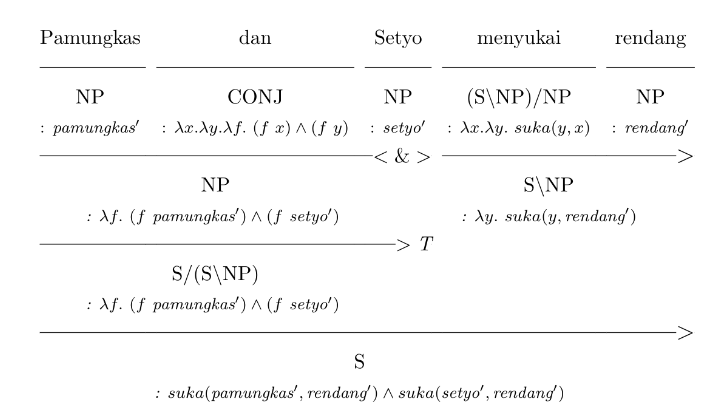
\includegraphics[width=.75\textwidth]{ccg1}
  \caption{
    Contoh CCG \textit{derivation} dengan operasi \textit{coordination},
    \textit{forward application}, dan \textit{type rising}.}
  \label{ccg-fig1}
\end{figure}

\begin{equation}\label{ccg:query:1}
  suka(\so{pamungkas}, \so{rendang}) \land suka(\so{setyo}, \so{rendang})
\end{equation}
\\


\noindent\textbf{Lambda Calculus}

\textit{Lambda calculus} ({$\lambda$}\textit{-calculus}) merupakan sebuah formalisme yang dikembangkan
oleh Alonzo Church sebagai alat yang digunakan untuk memahami konsep komputasi yang efektif
\citep{DBLP:journals/corr/Rojas15}.
Formalisme {$\lambda$}\textit{-calculus} cukup populer dan bahkan dijadikan sebagai pondasi teori bagi
paradigma pemrograman \textit{functional programming}.
Konsep utama dari {$\lambda$}\textit{-calculus} adalah apa yang disebut dengan \textit{expression}.
Suatu \textit{expression} dalam {$\lambda$}\textit{-calculus} terdiri dari tiga bagian yaitu
\textit{lambda notation} ({$\lambda$}), \textit{argument} (seperti $a$, $b$, $c$, $x$, dan lain-lain),
dan \textit{body} yang dipisahkan dengan tanda titik.
Sebagai contoh, fungsi lambda ${\lambda}x. x$ merupakan sebuah fungsi identitas yang mengambil
argumen $x$ kemudian mengembalikan nilai $x$ itu sendiri.
Dalam hal ini, terlihat bahwa notasi {$\lambda$} merupakan sebuah penanda bagi suatu fungsi lambda.
Kemudian, pengubah $x$ setelah notasi {$\lambda$} merupakan argumen dari fungsi tersebut.
Selanjutnya, tanda titik merupakan pemisah antara \textit{head} dan \textit{body} fungsi lambda.
Terakhir, setelah tanda titik adalah \textit{body} dari suatu fungsi lambda yang mana berupa
\textit{expression}.

Untuk mempermudah pemahaman, {$\lambda$}\textit{-calculus} dapat diperlakukan seperti fungsi tanpa
nama. Sebagai contoh, fungsi lambda $({\lambda}x. x + 5)$ apabila diberikan nilai $2$ sehingga
menjadi $({\lambda}x. x + 5) 2$ akan dievaluasi menjadi ${\lambda}(2). (2) + 5$.
Demikian itu, nilai yang dikembalikan oleh fungsi tersebut adalah $7$.
Sama seperti fungsi pada umumnya, konsep ini bernama \textit{substition} (substitusi).
Memahami {$\lambda$}\textit{-calculus} dirasa perlu berhubung dalam tugas akhir ini
{$\lambda$}\textit{-calculus} digunakan sebagai bentuk formal di \textit{category}
dalam konteks CCG \textit{lexicon}. Meskipun {$\lambda$}\textit{-calculus} tidak sesederhana
yang dijelaskan sebelumnya, setidaknya memahami {$\lambda$}\textit{-calculus} seperti ini
sudah cukup untuk dapat membangun \textit{supertagger} yang ada di tugas akhir ini.
\\


\noindent\textbf{CCGweb}

CCGweb\footnote{\url{https://github.com/texttheater/ccgweb}} merupakan
\textit{open source graphical annotation tool} pertama untuk CCG \citep{evang-etal-2019-ccgweb}.
Aplikasinya berbasis web dan dibangun dengan menggunakan bahasa pemrograman
Python, PHP, dan JavaScript.
Fitur yang paling menarik dari \textit{graphical annotation tool} adalah What You See Is What
You Get (WYSIWYG) yang mana berupa kemampuan untuk me-\textit{render} CCG \textit{derivation}
sesuai dengan apa yang kita lihat.
Maksudnya, CCG \textit{derivation} akan ditampilkan horizontal sesuai dengan panjang kalimatnya
kemudian hasil \textit{derivation}-nya ditampilkan vertikal seperti contoh pada
Bagian \ref{kajian-ccg}.

Untuk dapat menggunakan CCGweb, kita perlu melakukan instalasi terlebih dahulu.
Selanjutnya barulah kita dapat menambahkan kalimat-kalimat yang ingin dianotasi.
Satu instalasi CCGweb hanya dapat digunakan untuk satu proyek anotasi sehingga
apabila kita memiliki lebih dari satu proyek maka kita perlu melakukan instalasi
CCGweb yang baru.
Demikian itu, CCGtown\footnote{\url{https://github.com/wisn/ccgtown}} hadir dengan
fitur \textit{multi-project} dan tanpa perlu melakukan instalasi di komputer lokal
karena aplikasinya \textit{hosted} sehingga dapat diakses kapan pun.



\section{Sistem yang Dibangun}

CCGtown dibangun dengan menggunakan bahasa pemrograman Python dan JavaScript.
Adapun \textit{framework} yang digunakan adalah Django.
Versi awal CCGtown merupakan sebuah \textit{proof-of-concept} dari
\textit{open source graphical annotation tool} berbasis web yang dilengkapi dengan fitur
penganotasian semi-otomatis.
Bahasa pemrograman Python digunakan karena sebagian besar \textit{library} untuk CCG
sudah tersedia di PyPi \footnote{\url{https://pypi.org/}}.
Salah satu \textit{library} penting yang digunakan sebagai dasar dari fitur penganotasian
semi-otomatis adalah NTLK \footnote{\url{http://www.nltk.org/}}.
Selanjutnya, Django digunakan untuk mempercepat proses pengembangan aplikasi.
Adapun JavaScript digunakan untuk menjadikan CCGtown aplikasi berbasis web yang interaktif.

Alur kerja CCGtown pada umumnya adalah (1) pengguna melakukan registrasi, (2) pengguna
melakukan \textit{login} ke sistem, (3) pengguna membuat proyek baru, (4) pengguna
menambahkan kalimat yang ingin dianotasi, (5) pengguna melakukan anotasi kemudian melakukan
\textit{generate} CCG \textit{derivation} dan/atau melakukan modifikasi
\textit{derivation}-nya apabila diperlukan, dan (6) pengguna melakukan \textit{export}
setelah selesai melakukan anotasi. Alur kerja tersebut mempengaruhi desain sistem dari
CCGtown. Salah satunya adalah desain dari \textit{database} yang akan digunakan.
\\


\noindent\textbf{Desain Database}

CCGtown menggunakan PostgreSQL sebagai
DBMS\footnote{Database Management System}-nya.
Hal ini karena PostgreSQL memiliki kemampuan untuk menyimpan struktur data
JSON\footnote{JavaScript Object Notation} sehingga memudahkan CCGtown untuk menyimpan
format JSON dari CCG \textit{derivation} yang telah dimanipulasi oleh pengguna melalui
fitur \textit{editable CCG derivation}.
PostgreSQL juga memiliki banyak fitur lain termasuk di antaranya dukungan
dari \textit{non-relational database model} (seperti \textit{multi-model graph})
sehingga apabila di waktu yang akan datang CCGtown memerlukan perubahan signifkan
terhadap desain \textit{database}-nya tidak perlu mengganti DBMS yang digunakan
\citep{schonig2018mastering}.
Fitur lain seperti \textit{function} dan \textit{procedure} juga akan sangat membantu
pengembangan CCGtown di waktu yang akan datang.

CCGtown versi awal sejatinya hanya membutuhkan tiga tabel saja yaitu tabel
\textit{accounts} untuk menyimpan pengguna yang terdaftar, tabel
\textit{projects} untuk menyimpan proyek-proyek yang sudah dibuat, dan tabel
\textit{sentences} untuk menyimpan kalimat-kalimat yang akan dianotasikan.
Tiga tabel tersebut sudah cukup untuk membangun \textit{proof-of-concept} dari
alat anotasi CCG yang akan dibangun. Adapun
ERD\footnote{Entity Relationship Diagram}-nya dapat dilihat pada Gambar\ref{erd-1}.

\begin{figure}\centering\small
  \scalebox{.75}{
  \begin{tikzpicture}[node distance=1.5cm, every edge/.style={link}]
    \node[entity] (acc) {Accounts};
    \node[attribute] (acc-id) [above=of acc] {\key{ID}} edge (acc);
    \node[attribute] (acc-uuid) [above right=of acc] {\key{UUID}} edge (acc);
    \node[attribute] (acc-email) [right=of acc] {Email} edge (acc);
    \node[attribute] (acc-password) [below right=of acc] {Password} edge (acc);

    \node[relationship] (creates) [left=of acc] {Creates} edge (acc);

    \node[entity] (prj) [below=of creates] {Projects} edge (creates);
    \node[attribute] (prj-id) [above right=of prj] {\key{ID}} edge (prj);
    \node[attribute] (prj-uuid) [above left=of prj] {\key{UUID}} edge (prj);
    \node[attribute] (prj-author) [left=of prj] {Author ID} edge (prj);
    \node[attribute] (prj-name) [below left=of prj] {Name} edge (prj);
    \node[attribute] (prj-status) [below=of prj] {Status} edge (prj);
    \node[attribute] (prj-rules) [below right=of prj] {Rules} edge (prj);

    \node[relationship] (adds) [right=0.5cm and 2cm of prj] {Adds} edge (prj);

    \node[entity] (snt) [below=of adds] {Sentences} edge (adds);
    \node[attribute] (snt-id) [left=of snt] {\key{ID}} edge (snt);
    \node[attribute] (snt-uuid) [below left=of snt] {\key{UUID}} edge (snt);
    \node[attribute] (snt-project) [below=of snt] {Project ID} edge (snt);
    \node[attribute] (snt-words) [below right=of snt] {Words} edge (snt);
    \node[attribute] (snt-cats) [right=of snt] {Categories} edge (snt);
    \node[attribute] (snt-deriv) [above right=of snt] {Derivations} edge (snt);
  \end{tikzpicture}
  }
  \caption{Conceptual Entity Relationship Diagram (ERD) CCGtown}
  \label{erd-1}
\end{figure}

Masing-masing tabel memiliki dua \textit{key} yaitu $ID$ dan
$UUID$\footnote{Universally Unique IDentifier}.
$ID$ merupakan \textit{primary key} \textit{integer} dengan \textit{auto increment}
yang berfungsi sebagai \textit{identifier} untuk melakukan operasi
\textit{update} maupun \textit{delete}.
Adapun $UUID$ merupakan \textit{indexed column} yang berfungsi sebagai
\textit{indentifier} publik (dapat dilihat oleh pengguna melalui URL)
yang mana digunakan untuk operasi \textit{read}.
$ID$ tidak digunakan sebagai \textit{identifier} publik karena pengguna dapat
melakukan \textit{brute-force} untuk mencari proyek ataupun kalimat berdasarkan
$ID$ yang bukan miliknya.
Demikian itu alasan ditambahkannya atribut $UUID$.
Alasan kenapa CCGtown tetap menyimpan kolom $ID$ adalah karena $ID$ nantinya akan
digunakan untuk membuat \textit{pagination}.

Pada tabel $accounts$, selain $ID$ dan $UUID$ juga memiliki atribut $email$ dan
$password$. Masing-masing atribut tersebut menggunakan tipe data \textit{string}
atau VARCHAR di PostgreSQL.
Tabel $accounts$ memiliki hubungan \textit{one-to-many} terhadap tabel $projects$.
Adapun atribut tabel $projects$ adalah $author\_id$, $name$, $status$, dan $rules$.
Atribut $author\_id$ merupakan \textit{foreign key} (\textit{indexed}) yang
mengarah kepada tabel $accounts$ dan tipe data yang digunakan sama dengan
atribut $ID$ yang terdapat di tabel $accounts$.
Atribut $name$ menggunakan tipe data \textit{string} (VARCHAR).
Atribut $status$ menggunakan tipe data \textit{integer} yang berperan sebagai
\textit{enum} ($0$ = \textit{just created}, $1$ = \textit{in progress},
$2$ = \textit{finished}, dan $3$ = \textit{dropped}).
Tabel $projects$ memiliki hubungan \textit{one-to-many} terhadap tabel $sentences$.
Adapun atribut tabel $sentences$ adalah $project\_id$, $words$, $categories$, dan
$derivations$. Atribut $project\_id$ merupakan \textit{foreign key}
(\textit{indexed}) yang mengarah kepada tabel $projects$ dan tipe data yang digunakan
sama dengan atribut $ID$ yang terdapat di tabel $projects$.
Sisanya, atribut $words$, $categories$, dan $derivations$ menggunakan tipe data JSON.
\\


\noindent\textbf{Desain Sistem}

CCGtown sejatinya memiliki desain sistem yang cukup sederhana.
Fungsionalitas yang akan didukung untuk versi awal adalah (1) \textit{register} dan
\textit{login}, (2) manajemen proyek (CRUD\footnote{Create, Read, Update, Delete}
), (3) dan manajemen kalimat (CRUD).
Pada manajemen kalimat, CCGtown menggunakan JavaScript untuk membuat pembuatan
maupun perubahan CCG \textit{derivation} menjadi lebih interaktif.
Selain tiga fungsionalitas tersebut, CCGtown juga menambahkan fungsionalitas tambahan
seperti \textit{auto-assign category} yang dilakukan di sisi \textit{frontend}.
Kemudian, CCGtown juga menambahkan fungsionalitas tambahan di sisi \textit{backend}
yaitu CCG \textit{derivation generator} dengan memanfaatkan \textit{library} NLTK\citep{NTLKbook}
dan kemampuan untuk melakukan \textit{export} CCG \textit{derivation} yang disimpan
di \textit{database}.

Pengguna harus terdaftar terlebih dahulu sebelum dapat melaukan anotasi sehingga
langkah awal yang harus dibangun adalah fungsionalitas \textit{register}.
Alur proses pendaftaran pengguna dapat dilihat pada Gambar \ref{flowchart:register}.
Berhubung fokus saat ini adalah \textit{proof-of-concept}, informasi yang dibutuhkan
untuk mendaftar hanyalah \textit{email} dan \textit{password}. Adapun
\textit{password confirmation} digunakan untuk memvalidasi \textit{password}
sehingga dapat mengurangi risiko pengguna melupakan
\textit{password}-nya yang baru saja di-\textit{input}.
Saat pengguna melakukan pendaftaran, sistem akan memeriksa apakah \textit{email} yang
didaftar sudah terdapat di \textit{database}.
Apabila sudah terdaftar, pengguna akan dialihkan ke halaman \textit{register} kembali
dan mendapatkan \textit{flash message} dengan keterangan "email sudah terdaftar".
Sebaliknya, sistem akan melakukan \textit{input} data tersebut ke dalam \textit{database}
lalu mengalihkan pengguna ke halaman \textit{login}.
Ketika dialihkan ke halaman \textit{login}, pengguna akan melihat \textit{flash message}
dengan keterangan "pengguna berhasil didaftarkan".
Pada tahap ini pengguna sudah dapat melakukan \textit{login} ke dalam sistem CCGtown.

\begin{figure}\centering\small
  \scalebox{.75}{
	\begin{tikzpicture}[node distance=2cm]
    \node (start) [cloud] {Start};
    \node (input) [io, below of=start, yshift=0.5cm] {\textit{Input email, password,} dan \textit{password confirmation}};
    \node (check) [process, below of=input, yshift=0.5cm] {Mencari pengguna berdasarkan \textit{email}};
    \node (is-registered) [decision, below of=check, yshift=-1.25cm] {\textit{Email} sudah terdaftar?};
    \node (registered) [process, right of=is-registered, yshift=0cm, xshift=4.5cm] {\textit{Redirect} ke halaman \textit{register}};
    \node (registering) [process, below of=is-registered, yshift=-1.75cm] {\textit{Input} informasi pengguna ke \textit{database}};
    \node (redirect) [process, below of=registering, yshift=0.5cm] {\textit{Redirect} ke halaman \textit{login}};
    \node (stop) [cloud, below of=redirect, yshift=0.5cm] {Stop};

    \draw [arrow] (start) -- (input);
    \draw [arrow] (input) -- (check);
    \draw [arrow] (check) -- (is-registered);
    \draw [arrow] (is-registered) -- node[anchor=south]{Ya} (registered);
    \draw [arrow] (registered) -- +(3,0) |- (input);
    \draw [arrow] (is-registered) -- node[anchor=east]{Tidak} (registering);
    \draw [arrow] (registering) -- (redirect);
    \draw [arrow] (redirect) -- (stop);
  \end{tikzpicture}
  }
	\caption{Alur proses pendaftaran pengguna.}
  \label{flowchart:register}
\end{figure}

Pada proses "\textit{input} informasi pengguna ke \textit{database}" CCGtown melakukan
\textit{password hashing} dengan menggunakan Bcrypt.
Informasi sensitif seperti \textit{password} sebaiknya tidak disimpan sebagai
\textit{plain text}. Demikian itu CCGtown menggunakan \textit{password hashing}.
Apabila hal buruk terjadi seperti misalnya \textit{data breach} (kebocoran data),
\textit{password} pengguna tidak dapat langsung digunakan.
Peretas perlu mencari cara untuk memecahkan \textit{password} tersebut.
Bcrypt merupakan skema \textit{password hashing} berbasis Blowfish \textit{block cipher}
yang didesain untuk lebih \textit{resistant} terhadap serangan \textit{brute-force}
\citep{bcrypt}.
Serangan \textit{brute-force} merupakan upaya peretas untuk menebak \textit{password}
dengan cara membuat \textit{wordlist} yang kemudian dicocokkan dengan \textit{hash}
yang terbentuk satu-demi-satu.
Meskipun terjadi \textit{data breach}, peretas perlu usaha ekstra untuk dapat menebak
\textit{password} dari satu pengguna.
Hal ini mengurangi kerugian yang akan dialami oleh CCGtown apabila \textit{data breach}
benar-benar terjadi.

Selanjutnya, setelah melakukan registrasi, pengguna dapat melakukan \textit{login} ke
sistem CCGtown.
Proses yang dilakukan pada umumnya sama dengan aplikasi web yang memiliki
kemampuan \textit{register} dan \textit{login}. Alur proses \textit{login} dapat dilihat
pada Gambar \ref{flowchart:login}.
Setelah pengguna melakukan \textit{input} \textit{email} dan \textit{password}-nya,
CCGtown akan melakukan pencarian di \textit{database} apakah \textit{email} yang
diberikan terdaftar. Apabila tidak terdaftar, pengguna akan dialihkan ke halaman
\textit{login} dan diberikan \textit{flash message} "\textit{Email} dan/atau
\textit{password} tidak cocok". Pesan ini diberikan agar peretas tidak dapat mencari
tahu \textit{email} mana saja yang sudah terdaftar. Selanjutnya, apabila akun
dengan \textit{email} tersebut ada, maka langkah selanjutnya adalah mencocokkan
\textit{password} yang diberikan oleh pengguna dan \textit{password} yang telah
disimpan di \textit{database}. Kemudian, sistem melakukan Bcrypt \textit{sync}.
Apabila tidak berhasil, pengguna akan dialihkan ke halaman \textit{login}
dan diberikan \textit{flash message} "\textit{Email} dan/atau \textit{password}
tidak cocok". Sebaliknya, pengguna akan dialihkan ke halaman Projects yang berisi
daftar proyek yang telah dibuat sebelumnya.

\begin{figure}\centering\small
  \scalebox{.75}{
	\begin{tikzpicture}[node distance=2cm]
    \node (start) [cloud] {Start};
    \node (input) [io, below of=start, yshift=0.5cm] {\textit{Input email} dan \textit{password}};
    \node (check) [process, below of=input, yshift=0.5cm] {Mencari pengguna berdasarkan \textit{email}};
    \node (is-registered) [decision, below of=check, yshift=-1.25cm] {\textit{Email} sudah terdaftar?};
    \node (not-registered) [process, left of=is-registered, yshift=0cm, xshift=-4.5cm] {\textit{Redirect} ke halaman \textit{login}};
    \node (logging-in) [process, below of=is-registered, yshift=-1.75cm] {Mencocokkan \textit{password} dengan Bcrypt \textit{sync}};
    \node (is-matched) [decision, below of=logging-in, yshift=-1.25cm] {\textit{Password} cocok?};
    \node (redirect) [process, below of=is-matched, yshift=-1.75cm] {\textit{Redirect} ke halaman Projects};
    \node (stop) [cloud, below of=redirect, yshift=0.5cm] {Stop};

    \draw [arrow] (start) -- (input);
    \draw [arrow] (input) -- (check);
    \draw [arrow] (check) -- (is-registered);
    \draw [arrow] (is-registered) -- node[anchor=south]{Tidak} (not-registered);
    \draw [arrow] (not-registered.north) -- +(0,0) |- (input);
    \draw [arrow] (is-registered) -- node[anchor=east]{Ya} (logging-in);
    \draw [arrow] (logging-in) -- (is-matched);
    \draw [arrow] (is-matched.west) -| +(-4.9,0) -- node[anchor=east]{Tidak} (not-registered.south);
    \draw [arrow] (is-matched) -- node[anchor=east]{Ya} (redirect);
    \draw [arrow] (redirect) -- (stop);
  \end{tikzpicture}
  }
	\caption{Alur proses \textit{login} ke sistem CCG.}
  \label{flowchart:login}
\end{figure}

Pada halaman Projects, pengguna dapat membuat proyek atau menghapus proyek.
Tidak ada fungsionalitas spesial di halaman Projects selain CRUD pada umumnya.
Satu pengguna dapat membuat banyak proyek. Tidak ada larangan tertentu terhadap penamaan
proyek. Namun, sangat disarankan memberikan nama proyek yang deskriptif seperti misalnya
"\textit{Wide-range Indonesian Dataset}". Setiap proyek memiliki status yang berbeda-beda.
Proyek yang baru saja dibuat akan memiliki status \textit{just created}.
Hal ini untuk memudahkan \textit{annotator} mencari proyek mana yang baru akan dikerjakan,
proyek mana yang sedang dikerjakan, proyek mana yang sudah selesai dikerjakan, atau
proyek mana yang tidak jadi dikerjakan. Proyek yang telah dibuat dapat disunting maupun
dihapus. Proyek yang dihapus tidak dapat dikembalikan (\textit{undo}).
Adapun penyuntingan proyek terjadi di halaman Editor.

Pada halaman Editor, pengguna dapat menyunting informasi proyek seperti nama proyek,
status proyek, dan \textit{rules} yang akan digunakan untuk melakukan \textit{generate}
CCG \textit{derivation} via NTLK. Selain itu, pengguna juga dapat menambahkan kalimat
baru yang akan dianotasi. Pengguna dapat menambahkan lebih dari satu kalimat sekaligus.
Kalimat-kalimat tersebut akan di-\textit{tokenize} menggunakan \textit{library} NLTK.
Ekstensi yang digunakan untuk proses \textit{tokenize} ini adalah punkt.
Setelah itu, barulah pengguna dapat melakukan penganotasian terhadap kalimat-kalimat yang
telah ditambahkan. Terdapat dua cara untuk memberikan anotasi yaitu secara langsung di
halaman Editor atau dapat juga dilakukan di Editable CCG Modal.
Saat ini CCGtown belum mendukung penganotasian terhadap \textit{compound words}.
CCGtown saat ini juga belum mendukung penganotasian CCG dengan semantik.
Versi awal CCGtown hanya mendukung penganotasian CCG secara sintaksis saja.

Setelah semua kata dalam suatu kalimat diberikan anotasi, pengguna dapat melakukan
\textit{generate} CCG \textit{derivation}. Hal ini dapat dilakukan berkat bantuan
\textit{library} NLTK. Kami mengambil sebuah $rules$ dari tabel $projects$ dan kemudian
kami mengambil semua $words$ serta $categories$ dari tabel $sentences$ yang merupakan
bagian dari proyek tersebut. Kolom $words$ merupakan kumpulan kata dari kalimat yang telah
di-\textit{tokenize}. Adapun kolom $categories$ merupakan anotasi CCG \textit{category}-nya.
\textit{Pseudocode} untuk \textit{generate} CCG \textit{derivation} dapat dilihat pada
Kode \ref{code:ccg-gen} dengan asumsi anotasi yang diberikan absah (dapat dibuat CCG
\textit{derivation}-nya). Kode $next$ tersebut akan mengambil satu dari banyak
kemungkinan \textit{derivation} yang dapat dibuat. Contoh \textit{object} yang
di-\textit{return} dapat dilihat pada Kode \ref{code:ccg-gen-example}.
Untuk kepentingan \textit{rendering} di sisi \textit{frontend}, \textit{key} seperti
$from$ dan $to$ sangat diperlukan. \textit{Key} $from$ dan \textit{key} $to$
merepresentasikan \textit{index} posisi terhadap \textit{array} $words$.
Dengan bantuan kedua \textit{key} tersebut, \textit{frontend} dapat melakukan kalkulasi
posisi masing-masing elemen yang terdapat di \textit{object} $derivations$.

\begin{lstlisting}[
  language=python,
  firstnumber=1,
  caption={Pseudocode untuk melakukan \textit{generate} CCG \textit{derivation}.},
  label={code:ccg-gen}
]
from nltk.ccg import chart, lexicon

def generateCCGDerivation(rules, words, categories, target_words):
    lex = rules + '\n\n'
    for i in range(len(words)):
        lex += words[i] + ' => ' + categories[i] + '\n'

    lex = lexicon.parseLexicon(lex)
    parser = chart.CCGChartParser(lex, chart.DefaultRuleSet)
    result = next(parser.parse(target_words))
    derivations = makeCCGDeriv(result)

    return derivations
\end{lstlisting}

Kode \ref{code:ccg-gen-example} didapatkan dari fungsi $makeCCGDeriv$ yang terdapat pada
Kode \ref{code:ccg-gen}. Fungsi $makeCCGDeriv$ sederhananya mengambil $Tree$ yang didapatkan
dari $parser.parse$ kemudian melakukan \textit{tree traversal}. Semua \textit{leaf}, diambil
dari paling "kiri", diletakkan di elemen pertama $derivations$. Selanjutnya, kita berjalan
melalui \textit{parent} dari \textit{leaf} tersebut hingga ke \textit{root} mencari bentuk CCG
\textit{derivation}-nya. Banyaknya baris yang dibutuhkan oleh CCG \textit{derivation} dapat
dilihat dari \textit{height} yang dimiliki oleh $Tree$ tersebut. Kemudian, hasil dari CCG
\textit{derivation} (umumnya berupa $S$) merupakan elemen terakhir $derivations$.

\begin{lstlisting}[
  language=json,
  firstnumber=1,
  caption={Contoh \textit{derivations object} yang di-\textit{return}.},
  label={code:ccg-gen-example}
]
[
  [
    { "to": 0, "from": 0, "word": "You" },
    { "to": 1, "from": 1, "word": "prefer" },
    { "to": 2, "from": 2, "word": "that" },
    { "to": 3, "from": 3, "word": "cake" }
  ],
  [
    { "to": 0, "from": 0, "category": "NP" },
    { "to": 1, "from": 1, "category": "((S\NP)/NP)" },
    { "to": 2, "from": 2, "category": "(NP/N)" },
    { "to": 3, "from": 3, "category": "N" }
  ],
  [
    { "to": 3, "from": 2, "category": "NP", "operator": ">" }
  ],
  [
    { "to": 3, "from": 1, "category": "(S\NP)", "operator": ">" }
  ],
  [
    { "to": 3, "from": 0, "category": "S", "operator": "<" }
  ]
]
\end{lstlisting}

Selain memiliki kemampuan untuk melakukan \textit{generate} CCG \textit{derivation},
CCGtown juga memiliki kemampuan untuk melakukan \textit{auto-assign} CCG \textit{category}.
Token kata yang sudah dianotasi oleh pengguna akan disimpan ke dalam suatu \textit{dictionary}.
Untuk setiap kata yang belum dianotasi, CCGtown akan memeriksa apakah token kata tersebut
sebelumnya sudah dianotasi. Apabila sudah, CCGtown akan memberikan anotasi secara otomatis.
Suatu token kata mungkin memiliki lebih dari satu anotasi. CCGtown hanya akan mengambil satu
anotasi saja. Akibatnya, pengguna sebaiknya tetap melakukan peninjauan.
Kendati demikian, setidaknya kegiatan anotasi yang repetitif dapat berkurang sehingga memudahkan
dan mempercepat proses anotasi.


\noindent\textbf{Deployment}

CCGtown menggunakan Heroku sebagai \textit{cloud application platform} untuk \textit{hosting}
aplikasi tersebut agar dapat diakses oleh pengguna via internet. Heroku memberikan kemudahan
untuk melakukan \textit{deployment} dan \textit{scaling} apabila dibutuhkan
\citep{middleton2013heroku}. Selain itu, integrasi Heroku dengan GitHub memberikan fitur
\textit{automatic deployment} ke \textit{branch} tertentu sehingga pengembang tidak perlu
melakukan instalasi manual secara repetitif. Demikian itu, pengembang tidak akan direpotkan
dengan proses \textit{deployment}. Apa yang perlu dilakukan adalah melakukan \textit{setup}
terlebih dahulu kemudian \textit{automatic deployment} dapat berjalan sampai dengan dimatikan
kembali.

CCGtown menggunakan \textit{web framework} yang proses \textit{setup} dan \textit{run}-nya
dapat dijalankan hanya dengan beberapa perintah CLI\footnote{command line interface} saja.
Demikian itu, Heroku dapat menjalankan perintah-perintah tersebut dan ketika semua perintahnya
memberikan \textit{return value} berupa $0$ (sukses), secara otomatis Heroku akan menimpa
aplikasi yang sedang berjalan dengan yang baru. \textit{Dependency} NLTK seperti \textit{punkt}
juga tidak perlu di-\textit{install} manual. Hanya dengan menambahkan berkas "nltk.txt",
Heroku akan secara otomatis melakukan instalasi semua \textit{dependency} NLTK yang terdaftar di
berkas tersebut. Adapun \textit{dependency} untuk bahasa Python (PyPI) yang digunakan tersedia di
dalam berkas "requirements.txt" dan Heroku juga akan melakukan instalasi semua \textit{dependency}
yang terdaftar di dalam berkas tersebut.



\section{Evaluasi}

\subsection{Hasil Pengujian}

Pengujian dilakukan dengan menggunakan \textit{state transition testing} yang mana merupakan bagian
dari \textit{black-box testing}. Dalam hal ini, apa yang akan diuji adalah fungsionalitas dari
CCGtown dan \textit{testing} ini digunakan untuk mencari apakah ada \textit{bug} dari sistem yang
telah dibangun. Aturan \textit{state transition testing} cukup sederhana yaitu
(1) kunjungi setiap \textit{state}, (2) cakup semua transisi, dan (3) pastikan tidak ada
\textit{state} yang tak dapat dijangkau atau tak dapat dikembalikan\citep{black2016pragmatic}.
Untuk mempercepat proses pengujian, kami menggunakan \textit{state transition table} sebagai ganti
dari \textit{state transition diagram}. Daftar \textit{state} dapat dilihat pada Tabel
\ref{table:state-map}. Pada Tabel \ref{table:state-map}, S1 dan S2 merupakan \textit{initial state}
dan S5 merupakan \textit{final state}.

Pengujian dikelompokkan berdasarkan antarmuka yang dilihat oleh pengguna. Umumnya berupa halaman web
atau modal layar penuh. Masing-masing tabel memiliki kolom nomor, \textit{start state},
\textit{input}, \textit{output}, dan \textit{finish state}. Adapun transisi yang telah dikumpulkan
dapat dilihat pada Tabel \ref{table:register-page} untuk halaman registrasi, Tabel
\ref{table:login-page} untuk halaman login, Tabel \ref{table:project-page} untuk halaman proyek,
Tabel \ref{table:editor-page} untuk halaman editor, Tabel \ref{table:ccg-modal} untuk Editable CCG
Derivation Modal, dan Tabel \ref{table:conf-modal} untuk Configure Derivation Modal.


\subsection{Analisis Hasil Pengujian}

Pengguna dapat melakukan login secara langsung apabila telah memiliki akun sehingga dalam hal ini
\textit{state} S2 merupakan \textit{start state}. Sebaliknya, apabila belum memiliki akun, pengguna
dapat melakukan registrasi terlebih dahulu. Artinya, \textit{state} S1 juga merupakan
\textit{start state}. Tujuan CCGtown adalah untuk memfasilitasi \textit{annotator} dalam memberikan
anotasi CCG. Demikian itu, \textit{final state} CCGtown terdapat pada fitur \textit{export to} JSON
yang mana merupakan \textit{state} S5.

Pada Tabel \ref{table:register-page}, pengguna akan diarahkan ke \textit{state} selanjutnya yaitu
S2 ketika \textit{email} yang didaftarkan belum terdaftar dan \textit{password} yang diberikan absah
saja. Selain itu, pengguna akan dikembalikan ke \textit{state} S1 karena aksi yang dilakukan
sebelumnya tidak berhasil dilakukan. Adapun pada Tabel \ref{table:login-page}, penggunaan akan
diarahkan ke halaman proyek yang mana merupakan \textit{state} S3 ketika \textit{email} terdaftar
dan \textit{password} yang diberikan sesuai dengan yang didaftarkan sebelumnya. Selain itu,
pengguna akan diarahkan kembali ke halaman login.

Pada Tabel \ref{table:project-page}, ada cukup banyak hal yang dapat dilakukan oleh penggunaan.
Mulai dari \textit{logout} dari CCGtown, menambahkan proyek baru, menghapus suatu proyek, hingga
melakukan \textit{export to} JSON. Selanjutnya, apabila pengguna memutuskan untuk melihat atau
meng-\textit{edit} suatu proyek, ia akan diarahkan ke halaman editor yang mana merupakan
\textit{state} S4. Pada Tabel \ref{table:editor-page}, hanya ada dua transisi yang memiliki
\textit{finish state} selain S4 yaitu pada nomor 1, 11, dan 14. Selain ketiga transisi tersebut,
pengguna tetap berada di \textit{state} S4 yaitu halaman editor. Pengguna juga dapat langsung
menuju \textit{final state} dengan mengklik \textit{export to JSON} pada menu yang sudah tersedia.
Adapun transisi yang lain adalah aksi \textit{logout} dan aksi \textit{view ccg derivation} yang
mana akan membuka Editable CCG Derivation Modal (\textit{state} S6).

Pada Tabel \ref{table:ccg-modal}, pengguna dapat mengubah anotasi CCG dan dapat mengubah
penurunan CCG. Selain itu, pengguna dapat keluar dari modal tersebut atau dapat mengatur penurunan
yang ada. Pengaturan dari penurunan tersebut dapat dilakukan di Configure Derivation Modal yang
mana merupakan \textit{state} S7. Pada Tabel \ref{table:conf-modal}, pengguna dapat menambah
atau menghapus konfigurasi penurunan CCG. Transisi lainnya adalah keluar dari modal tersebut atau
simpan konfigurasinya. Demikian itu, dilihat dari \textit{state transition table} yang ada, CCGtown
selalu dapat kembali ke \textit{state} sebelumnya.



\section{Kesimpulan}

Berdasarkan \textit{state transition testing}, transisi yang terjadi pada CCGtown dapat berjalan
maju (misal: dari S3 ke S4) atau pun dapat berjalan mundur (misal: dari S4 ke S2). Hal tersebut
memungkinkan pengguna untuk kembali ke \textit{initial state} dan berakhir di \textit{final state}.
Satu-satunya \textit{state} yang tidak memiliki transisi baik maju maupun mundur adalah S7
yaitu \textit{export to} JSON. Hal ini dikarenakan ketika pengguna mengklik tombol \textit{export},
tab baru di \textit{browser} pengguna akan terbuka sehingga akan ada setidaknya dua tab aplikasi
CCGtown yang terbuka. Demikian itu, ketika pengguna menutup halaman hasil \textit{export} tersebut
lalu membuka CCGtown kembali, secara otomatis \textit{state} aktif tidak lagi S7. Adapun
\textit{state}-nya dapat berupa S3 atau S4. Apabila sesi pengguna kadaluwarsa, \textit{state} yang
akan aktif adalah S2. Demikian itu, berdasarkan pengujian ini semua fungsionalitas CCGtown sudah
berjalan dengan baik dan dapat digunakan oleh pengguna tanpa masalah.
 


\bibliographystyle{abbrv}
\bibliography{references}

\section*{Lampiran}

\begin{table}
  \caption{\textbf{Pemetaan State}}
  \label{table:state-map}
  \centering
  \begin{tabular}{| c | l |}
    \hline
    \textbf{State} & \textbf{Keterangan} \\ [0.5ex]
    \hline
    S1 & Halaman registrasi pengguna \\
    S2 & Halaman login \\
    S3 & Halaman proyek \\
    S4 & Halaman editor \\
    S5 & Halaman export JSON \\
    S6 & Editable CCG Derivation Modal \\
    S7 & Configure Derivation Modal \\ [1ex]
    \hline
  \end{tabular}
\end{table}

\begin{table}
  \caption{\textbf{State transition pada halaman registrasi pengguna}}
  \label{table:register-page}
  \centering
  \begin{tabular}{| c | c | m{45mm} | m{45mm} | c |}
    \hline
    \textbf{No.} & \textbf{Start State} & \textbf{Input} & \textbf{Output} & \textbf{Finish State} \\ [0.5ex]
    \hline
    1 & S1 & invalid email atau invalid password & diarahkan ke halaman registrasi & S1 \\
    2 & S1 & email terdaftar & diarahkan ke halaman registrasi & S1 \\
    3 & S1 & email tidak terdaftar dengan invalid password & diarahkan ke halaman registrasi & S1 \\    
    4 & S1 & email tidak terdaftar dengan valid password & diarahkan ke halaman login & S2 \\ [1ex]
    \hline
  \end{tabular}
\end{table}

\begin{table}
  \caption{\textbf{State transition pada halaman login}}
  \label{table:login-page}
  \centering
  \begin{tabular}{|c | c | m{45mm} | m{45mm} | c |}
    \hline
    \textbf{No.} & \textbf{Start State} & \textbf{Input} & \textbf{Output} & \textbf{Finish State} \\ [0.5ex]
    \hline
    1 & S2 & email terdaftar dan password sesuai & diarahkan ke halaman proyek & S3 \\
    2 & S2 & email tidak terdaftar atau password salah & diarahkan ke halaman login & S2 \\ [1ex]
    \hline
  \end{tabular}
\end{table}

\begin{table}
  \caption{\textbf{State transition pada halaman proyek}}
  \label{table:project-page}
  \centering
  \begin{tabular}{|c | c | m{45mm} | m{45mm} | c |}
    \hline
    \textbf{No.} & \textbf{Start State} & \textbf{Input} & \textbf{Output} & \textbf{Finish State} \\ [0.5ex]
    \hline
    1 & S3 & mengklik ikon profil kemudian logout & diarahkan ke halaman login & S2 \\
    2 & S3 & mengklik nama proyek atau edit proyek & diarahkan ke halaman editor & S4 \\
    3 & S3 & mengklik "remove project" kemudian "cancel" & tidak terjadi apa-apa & S3 \\
    4 & S3 & mengklik "remove project" kemudian "remove" & diarahkan ke halaman proyek dan proyek yang dipilih terhapus & S3 \\
    5 & S3 & mengklik "create new project" kemudian "cancel" & tidak terjadi apa-apa & S3 \\
    6 & S3 & mengklik "create new project" kemudian "create project" dengan memasukkan nama proyek & diarahkan ke halaman proyek dan proyek baru dibuat & S3 \\
    7 & S3 & mengklik "export to JSON" & tab baru terbuka dan menampilkan hasil export & S5 \\
    8 & S3 & sesi pengguna kadaluwarsa atau pengguna belum login & diarahkan ke halaman login & S2 \\ [1ex]
    \hline
  \end{tabular}
\end{table}

\begin{table}
  \caption{\textbf{State transition pada halaman editor}}
  \label{table:editor-page}
  \centering
  \begin{tabular}{| c | c | m{45mm} | m{45mm} | c |}
    \hline
    \textbf{No.} & \textbf{Start State} & \textbf{Input} & \textbf{Output} & \textbf{Finish State} \\ [0.5ex]
    \hline
    1 & S4 & mengklik ikon profil kemudian logout & diarahkan ke halaman login & S2 \\
    2 & S4 & melakukan suatu perubahan kemudian mengklik "save" & diarahkan ke halaman editor dan semua perubahan disimpan & S4 \\
    3 & S4 & mengubah/menghapus anotasi di suatu kata & anotasi pada kata tersebut berubah & S4 \\
    4 & S4 & mengklik "add new sentences" kemudian klik cancel & tidak terjadi apa-apa & S4 \\
    5 & S4 & mengklik "add new sentences" kemudian klik "add sentences" setelah menuliskan kalimat/paragraf & kalimat-kalimat baru ditambahkan & S4 \\
    6 & S4 & mengklik "generate ccg derivation" kemudian klik "cancel" & tidak terjadi apa-apa & S4 \\
    7 & S4 & mengklik "generate ccg derivation" kemudian klik "generate now" dengan invalid lexicon & ccg derivation tidak di-generate & S4 \\
    8 & S4 & mengklik "generate ccg derivation" kemudian klik "generate now" dengan valid lexicon & ccg derivation di-generate & S4 \\
    9 & S4 & mengklik "remove sentence" kemudian klik "cancel" & tidak terjadi apa-apa & S4 \\
    10 & S4 & mengklik "remove sentence" kemudian klik "remove sentence" & kalimat tersebut dihapus & S4 \\
    11 & S4 & mengklik "view ccg derivation" & editable ccg modal terbuka & S6 \\
    12 & S4 & mengklik "remove project" kemudian klik "cancel" & tidak terjadi apa-apa & S4 \\
    13 & S4 & mengklik "remove project" kemudian klik "remove project" & proyek dihapus lalu diarahkan ke halaman proyek & S3 \\
    14 & S4 & mengklik "export to JSON" & tab baru terbuka dan menampilkan hasil export & S5 \\
    15 & S4 & mengklik "auto-assign category" kemudian klik "cancel" & tidak terjadi apa-apa & S4 \\
    16 & S4 & mengklik "auto-assign category" kemudian klik "auto-assign now" & kata yang belum dianotasi diberikan anotasi dari kata yang sama di kalimat lain & S4 \\
    17 & S4 & sesi pengguna kadaluwarsa atau pengguna belum login & diarahkan ke halaman login & S2 \\ [1ex]
    \hline
  \end{tabular}
\end{table}

\begin{table}
  \caption{\textbf{State transition pada Editable CCG Derivation Modal}}
  \label{table:ccg-modal}
  \centering
  \begin{tabular}{| c | c | m{45mm} | m{45mm} | c |}
    \hline
    \textbf{No.} & \textbf{Start State} & \textbf{Input} & \textbf{Output} & \textbf{Finish State} \\ [0.5ex]
    \hline
    1 & S6 & mengklik tombol "X" & editable ccg derivation modal ditutup & S4 \\
    2 & S6 & mengklik "add new row" & baris kosong baru ditambahkan & S6 \\
    3 & S6 & mengklik anotasi kemudian mengubah/menghapus anotasi & anotasi yang dipilih berubah & S6 \\
    4 & S6 & mengklik "configure derivation on this row" & configure derivation modal terbuka & S7 \\ [1ex]
    \hline
  \end{tabular}
\end{table}

\begin{table}
  \caption{\textbf{State transition pada Configure CCG Modal}}
  \label{table:conf-modal}
  \centering
  \begin{tabular}{| c | c | m{45mm} | m{45mm} | c |}
    \hline
    \textbf{No.} & \textbf{Start State} & \textbf{Input} & \textbf{Output} & \textbf{Finish State} \\ [0.5ex]
    \hline
    1 & S7 & mengklik tombol "X" atau "cancel & configure ccg modal ditutup & S6 \\
    2 & S7 & mengklik tombol "save" & perubahan disimpan kemudian modal ditutup & S6 \\
    3 & S7 & mengklik "add entry" & konfigurasi kosong baru ditambahkan & S7 \\
    4 & S7 & mengklik tombol dengan ikon tempat sampah & konfigurasi yang dipilih terhapus & S7 \\ [1ex]
    \hline
  \end{tabular}
\end{table}
